\PassOptionsToPackage{x11names}{xcolor}
\documentclass[10pt]{beamer}

\usepackage{fontspec}
\setmainfont{Ubuntu}[]
\setsansfont{Ubuntu}[]
\setmonofont{Ubuntu Mono}[]

\usepackage{graphicx}
\graphicspath{ {../img/} }

\usepackage[absolute,overlay]{textpos} % [showboxes]

\beamertemplatenavigationsymbolsempty

\title{Defensive Programming vs Let It Crash}

\begin{document}

\begin{frame}
  \frametitle{Defensive Programming}
  Предвидеть все возможные ошибки.
  \par \bigskip
  Явно их обрабатывать.
\end{frame}

\begin{frame}
  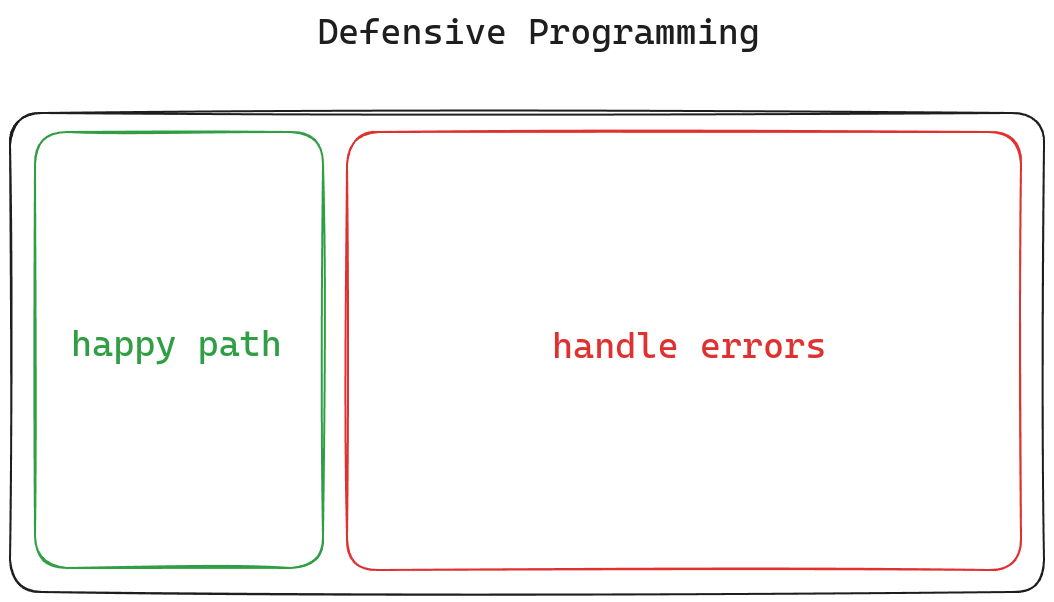
\includegraphics[scale=0.29]{defensive-programming}
\end{frame}

\begin{frame}
  \frametitle{Let It Crash}
  Уметь восстанавливаться после ошибок.
  \par \bigskip
  Не обрабатывать их явно.
\end{frame}

\begin{frame}
  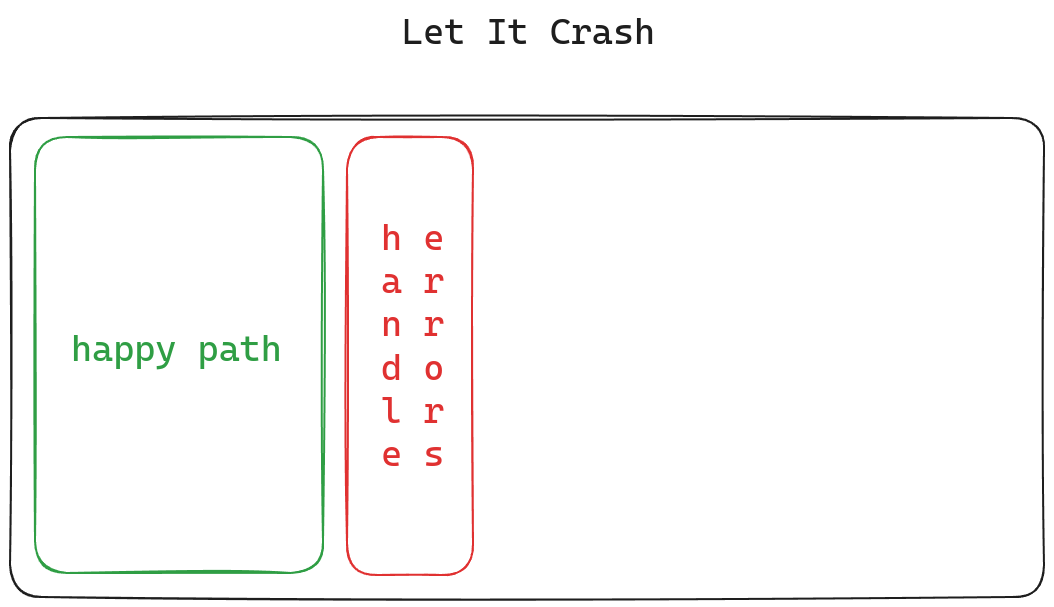
\includegraphics[scale=0.29]{let-it-crash}
\end{frame}

\begin{frame}
  \frametitle{Частота применения исключений}
  В разных языках разное отношение к применению исключений.
  \par \bigskip
  Где-то их вообще нет, как в Rust.
  \par \bigskip
  Где-то применяются на каждом шагу, как в Python.
\end{frame}

\begin{frame}
  \frametitle{Частота применения исключений}
  Сравним популярные библиотеки разных языков:
  \begin{itemize}
  \item Erlang: Cowboy
  \item Elixir: Ecto
  \item Python: Django
  \end{itemize}
\end{frame}

\begin{frame}
  \frametitle{Erlang: Cowboy 2.6.3}
  Библиотеки: cowboy, cowlib, ranch.
  \par \bigskip
  25К строк кода.
  \par \bigskip
  180 раз применяются исключения.
  \par \bigskip
  1 исключение на 260 строк кода.
\end{frame}

\begin{frame}
  \frametitle{Elixir: Ecto 3.3.2}
  28К строк кода.
  \par \bigskip
  300 раз применяются исключения.
  \par \bigskip
  1 исключение на 90 строк кода.
\end{frame}

\begin{frame}
  \frametitle{Python: Django 3.2}
  376К строк кода.
  \par \bigskip
  20K раз применяются исключения.
  \par \bigskip
  1 исключение на 20 строк кода.
\end{frame}

\begin{frame}
  \frametitle{Частота применения исключений}
  \centering
  Итого:
  \par \bigskip
  \setlength{\tabcolsep}{2em}
  \begin{tabular}{| l | l | r |}
    \hline
    Erlang & Cowboy & 1/260 \\
    \hline
    Elixir & Ecto & 1/90 \\
    \hline
    Python & Django & 1/20 \\
    \hline
  \end{tabular}
\end{frame}

\begin{frame}
  \centering
  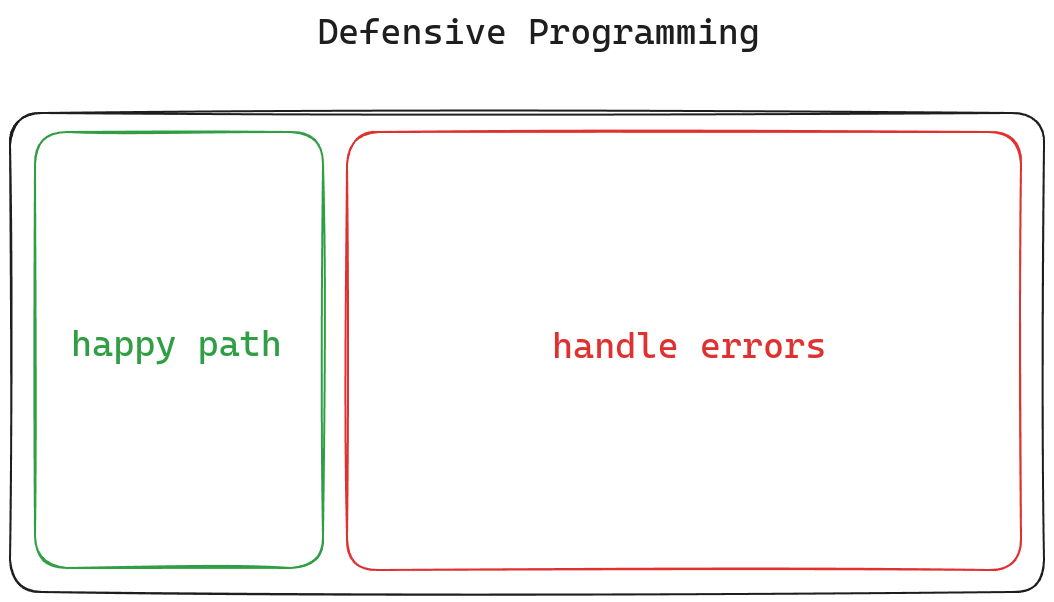
\includegraphics[scale=0.16]{defensive-programming}
  \par \bigskip
  \par \bigskip
  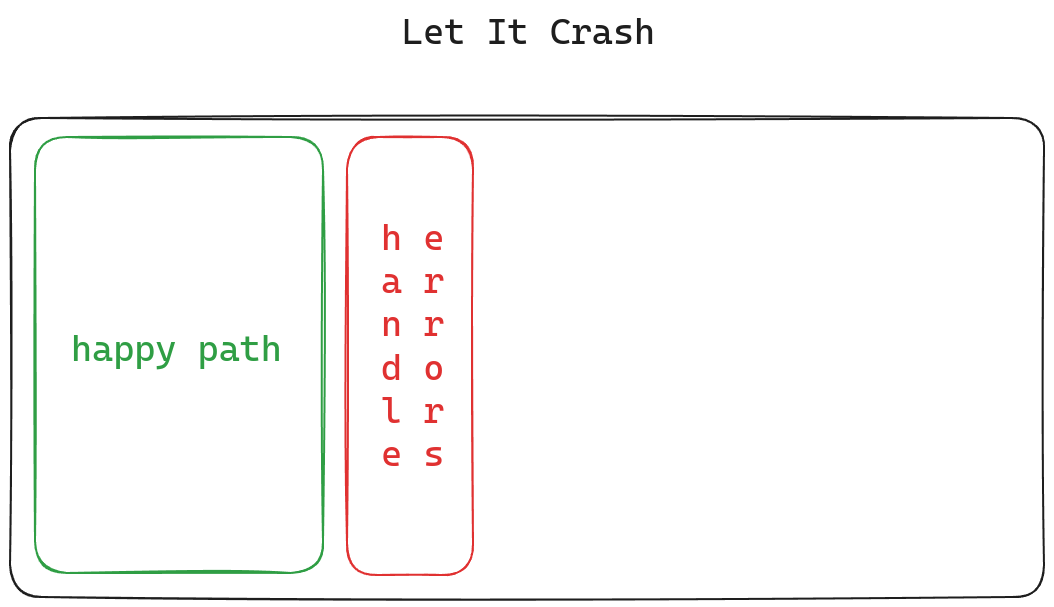
\includegraphics[scale=0.16]{let-it-crash}
\end{frame}

\end{document}
